\def\year{2018}\relax
%File: formatting-instruction.tex
\documentclass[letterpaper]{article} %DO NOT CHANGE THIS
\usepackage{aaai18}  %Required
\usepackage{times}  %Required
\usepackage{helvet}  %Required
\usepackage{courier}  %Required
\usepackage{url}  %Required
\usepackage{graphicx}  %Required
\frenchspacing  %Required
\setlength{\pdfpagewidth}{8.5in}  %Required
\setlength{\pdfpageheight}{11in}  %Required
\usepackage{spverbatim}
\usepackage{fancyvrb}

\usepackage{color}
\usepackage{xcolor}
\usepackage{amsmath,amsthm,stmaryrd}
\usepackage{algpseudocode}
\usepackage{algorithm}
\algrenewcommand\algorithmiccomment[2][\footnotesize]{{#1\hfill\(\triangleright\)
 #2}} %\normalsize
\usepackage{amssymb}
\usepackage{textcomp}

\usepackage{tikz}
\usetikzlibrary{shadows.blur}
\usetikzlibrary{shapes.symbols}
\usetikzlibrary{arrows,shapes,decorations.pathmorphing}
\usetikzlibrary{positioning}
\usetikzlibrary{decorations.text}
\usetikzlibrary{decorations.pathmorphing}
\usetikzlibrary{mindmap,backgrounds}
\tikzstyle{class}=[ellipse,align=center,fill=green!25]
\tikzstyle{data}=[draw,rectangle,align=center,black!70]
\tikzstyle{att}=[rectangle,align=center,fill=brown!70!red]
\tikzstyle{hasaA} = 
[draw,densely dashed,-,black!70,decoration={snake,segment 
length=10,amplitude=1.5,post length=4}]
\tikzstyle{hasaC} = [>=stealth',draw,thick,-, black]
\tikzstyle{isa} = [>=o,draw,densely dotted,very thick,black!90]

\newcommand{\authornote}[3]{
  {\fbox{\sc 
  #1}:$\blacktriangleright$\textcolor{#2}{\small{#3}}$\blacktriangleleft$}%
}
\newcommand{\pds}[1]{\authornote{PDS}{purple}{#1}}
\newcommand{\pjs}[1]{\authornote{PJS}{red}{#1}}
\newcommand{\gkg}[1]{\authornote{GKG}{brown}{#1}}
\newcommand{\ddg}[1]{\authornote{DDG}{blue}{#1}}
\newcommand{\npr}[1]{\authornote{NPR}{orange}{#1}}

\newcommand{\minizinc}{\textsc{MiniZinc}}
\newcommand{\chuffed}{\textsc{Chuffed}}
\newcommand{\relonto}{\textsc{Rel2Onto}}

\newcommand{\etal}{\textit{et al.}}

\newcommand{\code}[1]{\texttt{#1}}

%PDF Info Is Required:

%  \pdfinfo{
%/Title (2018 Formatting Instructions for Authors Using LaTeX)
%/Author (AAAI Press Staff)}
\setcounter{secnumdepth}{2}  
 \begin{document}
% The file aaai.sty is the style file for AAAI Press 
% proceedings, working notes, and technical reports.
%
\title{Using Machine Learning and Constraint Programming to Solve the 
Relational-To-Ontology Mapping Problem}
\author{}
\maketitle
\begin{abstract}
The problem of integrating heterogeneous data sources in an ontology is of high 
relevance in the database field. Several techniques exist to approach this 
problem. Nonetheless, side constraints on the data integration cannot be easily 
integrated with these tools and thus the results may be inconsistent. We 
present a new approach that combines Machine Learning and 
Constraint Programming techniques, by modelling the data integration problem as 
a Steiner Tree Problem in a weighted graph. We show that through this approach 
we can achieve better precision, recall and speed compared to state-of-the-art 
approaches. We provide a comprehensive set of experiments supporting our 
findings.
\end{abstract}

\section{Introduction}
The problem of integrating heterogeneous data sources is a long standing issue 
in the database research field and is of high relevance in many real-world 
domains.
A common approach to tackle this problem is to design a global model and to
construct source descriptions which specify mappings between the sources and
the global model \cite{doan2012principles}.

In our case, we would like this global model to account
not only for structural properties of the original data sources, but also to 
include the semantics, which is usually implicitly present in the sources. In 
other words, we want to build a semantic model which describes the data sources 
in terms of concepts and relationships defined by an ontology 
\cite{Taheriyan2013}. Henceforth, we 
focus on a specific data integration problem: automatically mapping a new 
relational data source onto a user provided ontology.

\subsubsection{Example} Consider the situation where we have some simple 
relational database tables with columns $\langle$\textit{Surname, 
Workplace, Date, Location}$\rangle$, 
$\langle$\textit{Company, Event, Begin, Until, Location}$\rangle$ and 
$\langle$\textit{Name, D.O.B, Location}$\rangle$. We do not \textit{a priori} 
know whether ``Date'' is the date of birth or the date a persons started 
working in the first table; or whether the ``Location'' on the second table 
refers to the location of the event, or the address of the company. 
If we are given an ontology like the one in Fig. \ref{FIG:onto}, we would like 
to automatically map the new data sources to classes of the 
ontology.$\square$

In this paper we use Machine Learning techniques (ML) to learn mapping rules 
from already mapped instances. To this end we formulate the 
Relational-To-Ontology Mapping Problem (\relonto{})
as a Minimum Cost Steiner Tree Problem (STP) with side constraints 
\cite{deuna2016steiner}.

Firstly, we build an \emph{integration graph} which includes the 
attributes from the new source as well as ontology classes and properties. 
Secondly, we apply machine learning techniques to 
assign costs to its edges. 
Lastly, we use Constraint Programming (CP) to 
find a minimum cost Steiner Tree in the graph. The goal is to assign the costs 
on the edges in such a way that the resulting Steiner Tree is a valid semantic 
model for the new source. 

The contributions of this work are:
\begin{itemize}
	\item \ddg{TODO}
\end{itemize}

Section \ref{SEC:pw} presents the previous work done to achieve this task. 
Section \ref{SEC:problem} formally states the problem. 
In Section \ref{SEC:ML} we present how we convert the information given into a 
useful data representation. 
Section \ref{SEC:STP} shows how we model the problem as a STP, 
whereas Section \ref{SEC:CP} discusses how we implement the model in CP. 
Section \ref{SEC:Res} shows our results. 

\section{Previous Work \label{SEC:pw}}
\ddg{rewrite, add more}
One of the standard approaches to solve the relational-to-ontology (\relonto{})
mapping problem is to apply Knowledge Representation and Reasoning (KR)
techniques. The main idea of this approach is to exploit constraints specified 
within relational schemata and ontologies. Several mapping generation
tools based on this approach already exist, for example, BootOX, MIRROR,
COMA++ \cite{pinkel2016rodi}. The issue is though that constraints may be 
inconsistent or absent completely \ddg{Why?}. We suggest to use ML techniques 
to overcome this hurdle.

\cite{taheriyan2016learning} \ddg{Isn't this really similar??}

\section{Problem Statement \label{SEC:problem}}
We follow the definitions proposed by Doal \etal{} \cite{doan2012principles}.


\begin{figure}[ht]
\centering
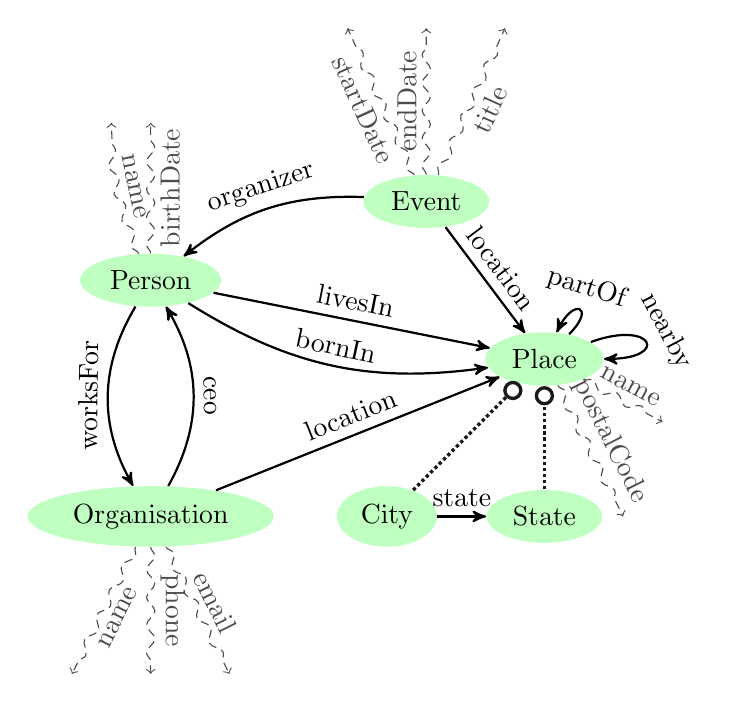
\begin{tikzpicture}
	\node[class] (pe) at (0,0)  {Person};
	\node[class] (co) at (0,-3) {Organisation};
	\node[class] (ev) at (3.5,1) {Event};
	\node[class] (pl) at (5,-1) {Place};
	\node[class] (ci) at (3,-3) {City};
	\node[class] (st) at (5,-3) {State};
	
		
	\path[hasaC,->] (pe) edge [bend left= -30] 
	node [midway, above, sloped] {worksFor} (co) ;
	\path[hasaC,->] (co) edge [bend left= -30] 
	node [midway, above, sloped] {ceo} (pe) ;
	
	\path[hasaC,->] (co) edge [] 
	node [midway, above, sloped] {location} (pl) ;
	
	\path[hasaC,->] (pe) edge [bend left = -20] 
	node [midway, above, sloped] {bornIn} (pl) ;
	\path[hasaC,->] (pe) edge [bend left = 0] 
	node [midway, above, sloped] {livesIn} (pl) ;
	
	\path[hasaC,->] (ev) edge [bend left = -20] 
	node [midway, above, sloped] {organizer} (pe) ;
	\path[hasaC,->] (ev) edge [bend left = 0] 
	node [midway, above, sloped] {location} (pl) ;
	
	
	\path[hasaC,->] (pl) edge [out=20,in=0,looseness=8] 
	node [midway, above, sloped] {nearby} (pl) ;
	\path[hasaC,->] (pl) edge [out=45,in=65,looseness=8] 
	node [midway, above, sloped] {partOf} (pl) ;
	
	\path[hasaC,->] (ci) edge  []
	node [midway, above, sloped] {state} (st) ;
	
	\path[isa,->] (ci) -- node [] {} (pl) ;
	\path[isa,->] (st) -- node [] {} (pl) ;
	

	\path[draw,hasaA,->] (pe) edge [decorate,bend left = 10] 
	node [midway, above, sloped] {name} (-0.5,2);
	\path[draw,hasaA,->] (pe) edge [decorate,bend left = 0] 
	node [midway, below, sloped] {birthDate} (0,2);	
	
	\path[draw,hasaA,->] (co) edge [decorate,bend left = 0] 
	node [midway, below, sloped] {name} (-1,-5);
	\path[draw,hasaA,->] (co) edge [decorate,bend left = 0] 
	node [midway, above, sloped] {phone} (0,-5);
	\path[draw,hasaA,->] (co) edge [decorate,bend left = 0] 
	node [midway, above, sloped] {email} (1,-5);
	
	\path[draw,hasaA,->] (ev) edge [decorate,bend left = 0] 
	node [midway, below, sloped] {startDate} (2.5,3.2);
	\path[draw,hasaA,->] (ev) edge [decorate,bend left = 0] 
	node [midway, above, sloped] {endDate} (3.5,3.2);
	\path[draw,hasaA,->] (ev) edge [decorate,bend left = 0] 
	node [midway, below, sloped] {title} (4.5,3.2);
	
	\path[draw,hasaA,->] (pl) edge [decorate,bend left = 0] 
	node [midway, above, sloped] {name} (6.5,-1.8);
	\path[draw,hasaA,->] (pl) edge [decorate,bend left = 0] 
	node [midway, above, sloped] {postalCode} (6,-3);	
	

\end{tikzpicture}
\caption{Example of ontology
(`\tikz{ \node[class] () at (0,0)  {};}' are Classes, `\tikz{ \path[hasaC,->] 
(0,1) -- (3ex,1);}' means ``has a Class property'', 
`\tikz{ \path[hasaA,decoration={post length=0}] (0,0) edge[decorate] (3ex,0);}' 
means ``has 
a data 
property'' and 
`\tikz{ \path[isa,->] (0,1) -- (3ex,1);}' means ``is a'' ). Based on 
\cite{Taheriyan2013}.
}
\label{FIG:onto}
\end{figure}




An ontology $\mathcal{O}$ is a specification of classes of objects, their 
data properties and relationships between them. An example of an ontology is 
given 
in Fig. \ref{FIG:onto}. A Class in an ontology can have \emph{data properties} 
or 
\emph{class properties}. For example an ``Organisation'' has a ``Person'' 
(which is a class with its own properties), and it has a ``name'' (which 
is a data property). Also, a Class can be a subclass of another Class. For 
example ``Cities'' and ``States'' are both ``Places''. A subclass 
inherits all the properties of the parent class.

A \emph{semantic model} $m$ is a directed graph with two types of nodes: 
\emph{class nodes} and \emph{data nodes}. We denote them as $\mathcal{C}_m$ and 
$\mathcal{D}_m$ respectively. We define $\mathcal{N}_m = \mathcal{C}_m \cup 
\mathcal{D}_m$. $ \mathcal{C}_m$ corresponds to classes in the ontology 
$\mathcal{O}$. $\mathcal{D}_m$ corresponds to data 
properties in the ontology. The edges in the semantic model correspond to 
relationships in the ontology, as shown if Figures \ref{FIG:onto} and 
\ref{FIG:sem}.



\begin{figure}[ht]
\centering
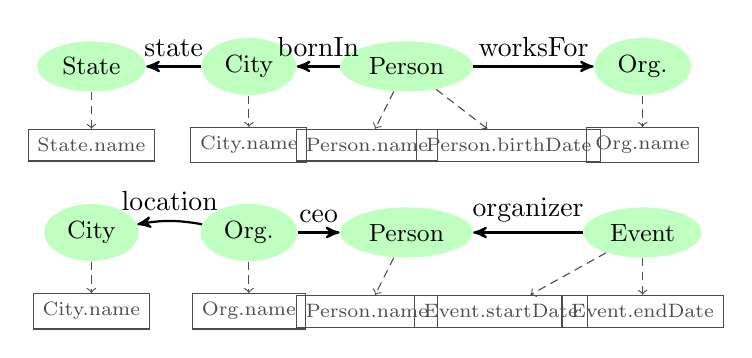
\begin{tikzpicture}
\begin{scope}
	\node[class] (pe) at (3,0)  {\small Person};
	\node[class] (co) at (6,0) {\small Org.};
	\node[class] (ci) at (1,0) {\small City};
	\node[class] (st) at (-1,0) {\small State};
	
	\node[data] (pen) at (2.5,-1) {\scriptsize Person.name};
	\node[data] (peb) at (4.3,-1) {\scriptsize Person.birthDate};
	\node[data] (cin) at (1,-1) {\scriptsize City.name};
	\node[data] (stn) at (-1,-1) {\scriptsize State.name};
	\node[data] (con) at (6,-1) {\scriptsize Org.name};
	
		
	\path[hasaC,->] (pe) edge [bend left= 0] 
	node [midway, above, sloped] {worksFor} (co) ;
	
	
	\path[hasaC,->] (pe) edge [bend left = 0] 
	node [midway, above, sloped] {bornIn} (ci) ;
	
	
	\path[hasaC,->] (ci) edge  []
	node [midway, above, sloped] {state} (st) ;

	

	\path[draw,hasaA,->] (pe) -- (pen);
	\path[draw,hasaA,->] (pe) -- (peb);	
	
	\path[draw,hasaA,->] (co) -- (con);
	
	\path[draw,hasaA,->] (ci) -- (cin);
	
	\path[draw,hasaA,->] (st) -- (stn);
\end{scope}
\begin{scope}[yshift=-60]
	\node[class] (pl) at (-1,0)  {\small City};
	\node[class] (pe) at (3,0)  {\small Person};
	\node[class] (co) at (1,0) {\small Org.};
	\node[class] (ev) at (6,0) {\small Event};
	
	\node[data] (pen) at (2.5,-1) {\scriptsize Person.name};
	\node[data] (evs) at (4.2,-1) {\scriptsize Event.startDate};
	\node[data] (eve) at (6,-1) {\scriptsize Event.endDate};
	\node[data] (con) at (1,-1) {\scriptsize Org.name};
	\node[data] (pln) at (-1,-1) {\scriptsize City.name};
	
		
	\path[hasaC,->] (co) edge [bend left= 0] 
	node [midway, above, sloped] {ceo} (pe) ;
	
	
	\path[hasaC,->] (ev) edge [bend left = 0] 
	node [midway, above, sloped] {organizer} (pe) ;
	
	\path[hasaC,->] (co) edge [bend left = -10] 
	node [midway, above, sloped] {location} (pl) ;



	\path[draw,hasaA,->] (pl) -- (pln);	

	\path[draw,hasaA,->] (pe) -- (pen);
	
	\path[draw,hasaA,->] (co) -- (con);
	
	\path[draw,hasaA,->] (ev) -- (evs);
	\path[draw,hasaA,->] (ev) -- (eve);
	
\end{scope}
\end{tikzpicture}
\caption{Examples of two semantic models (`\tikz{ \node[class] () at (0,0)  
{};}' are class nodes, and `\tikz{ \node[data] () at (0,0)  {};}' are data 
nodes).}
\label{FIG:sem}
\end{figure}




A \emph{source} $s$ is a $n$-ary relation with a set of attributes 
$\mathcal{A}_s = 
(a_1,...,a_n)$.

An \emph{attribute mapping} function $\phi : \mathcal{A}_s \mapsto 
\mathcal{D}_m$ is a function which
maps the attributes of the source $s$ into the nodes of the semantic model $m$. 
It can be a partial mapping, meaning that only some of the attributes
are connected to the nodes of $m$.

A \emph{source description} is a triple $\delta = (s, m, \phi)$ where $s$ is a 
source, 
$m$ is a semantic
model, and $\phi$ is an attribute mapping.

Our problem can be stated now the following way. We have an ontology 
$\mathcal{O}$ and a set of source descriptions $S_T = \{(s_1, m_1, \phi_1),..., 
(s_l, m_l, \phi_l)\}$.
Given a new source $s^\star$, we want to build a semantic model $m^\star$ and 
an attribute mapping function $\phi^\star$ such that 
$\delta^\star = (s^\star,m^\star,\phi^\star)$ is an \emph{appropriate} source 
description. We
use the term ``appropriate'' since there might be many such triples which are
well-formed source descriptions, but only one or a few will capture the intended
meaning of the source. Our goal is to automatically build $\delta^\star$ such 
that it minimizes the \emph{graph edit distance} (GED) from the semantic model 
$m^\star$ to the semantic model $m^\dag$ that the user considers correct.

The GED is a measure of similarity between two graphs defined as follows for 
two graphs $g_1$ and $g_2$: $GED(g_1,g_2) = min_{(e_1 ,...,e_k)\in P} 
\sum_{i=1}^{k}c(e_i)$ where $P$ denotes the set of edit paths transforming 
$g_1$ into (a graph
isomorphic to) $g_2$ and $c(e) \geq 0$ is the cost of each graph edit operation 
$e$. Graph edit operations include among others node insertion, edge deletion, 
etc. \cite{gao2010survey}. In practice, we use some approximation measures of 
the graph edit distance. \ddg{which approx?}

\section{ML for Training on Source Descriptions \label{SEC:ML}\ddg{Better title 
than this 
please...}}


\subsection{Semantic Labeling}
The semantic types $\mathcal{L_O} = \{l_1, l_2, ..., l_p\}$ of an ontology 
correspond to all pairs $(c,d)$, where $c$ is a Class in $\mathcal{O}$, and $d$ 
is a data property of that class (including inherited properties). 
For example, from the ontology in Fig. \ref{FIG:onto}, we would get types such 
as 
(City,name) and (State,name).

The first step to model the semantics of a new source $s^\star$ is to recognize 
the semantic types present in the source. 
We call this step \emph{semantic labeling}, which involves giving a confidence 
value to a match occurring between an attribute from $s^\star$ and type $l \in 
\mathcal{L_O}$. \ddg{CHECK!}

We formulate the problem of semantic labeling as a multi-class classification
problem. The known source descriptions $S_T$ provide us the training sample. We
compute a feature vector for each source \ddg{Which features?} attribute and 
associate the known
semantic type with the corresponding feature vector. We train a random forest
on this sample. Then we use the learnt model to classify attributes in the new
source.

In such way, we learn the mapping $\psi : \mathcal{A}_s \times \mathcal{L_O} 
\mapsto [0, 1]$,
where $\psi(a_i,l_j)$ indicates the confidence of the attribute $a_i$ to be 
mapped to the semantic type $l_j$.

\ddg{IMPORTANT: Do we keep all of them, or only the top $k$ with most 
confidence? If so, 
what is $k$?}



\subsection{Alignment Graph}

To provide an integrated view over the known sources descriptions $S_T$, we 
need to align their semantic models as well as all considered semantic 
types. This is achieved by constructing an \emph{alignment graph}. 

The alignment graph is a directed weighted graph $\mathcal{G_O} = 
(\mathcal{V_O},\mathcal{E_O})$ built on top 
of the known semantic models and expanded using the semantic types 
$\mathcal{L_O}$ and the ontology $\mathcal{O}$. Similar to a semantic 
model, $\mathcal{G_O}$ contains both class and data nodes. The links correspond 
to properties in  $\mathcal{O}$ and are weighted \cite{taheriyan2016learning}.

The algorithm we used to construct $\mathcal{G_O}$ is the same as Taheriyan 
\etal{} and is described in detail in the cited paper 
\cite{taheriyan2016learning}.
Briefly, the algorithm has three parts:
\begin{enumerate}
\item Adding the known semantic models.
\item Adding the semantic types learned for the target source. \ddg{TODO: see 
Important note above}
\item Expanding the graph using the domain ontology $\mathcal{O}$.
\end{enumerate}

Note how the alignment graph contains data nodes that correspond to at least 
some of the semantic types. For instance, it could contain two nodes 
$City.name$ and $State.name$ rather than just one node $name$ connected to two 
nodes $City$ and $State$. We say these nodes are \emph{induced} into the 
alignment graph by the semantic types, we note them $\mathcal{D_{G_O}}$ and we 
call them \emph{data nodes} of the alignment graph.

The graph is weighted by a function $w_\mathcal{O} : \mathcal{E_O} \mapsto 
\mathbb{R}$ in 
such a way that edges which are present in
the known semantic models have lower weights than those 
which are inferred from the ontology. As we will see int he next section, this 
makes edges present in semantic models more attractive. \ddg{How exactly are 
they weighted?}

An example alignment graph is illustrated in Fig. \ref{FIG:ali}. Bigger 
examples 
can be found in \cite{Taheriyan2013}. Black links 
correspond to the links which are supported by the known semantic models. Blue 
and orange links are inferred from the ontology $\mathcal{O}$ (the orange ones 
correspond to the ones added to connect Classes of the ontology that never 
appeared in the semantic models) and can be assigned the 
maximum weight $w_max$ \ddg{where does this weight come from?} .


\begin{figure}[ht]
\centering
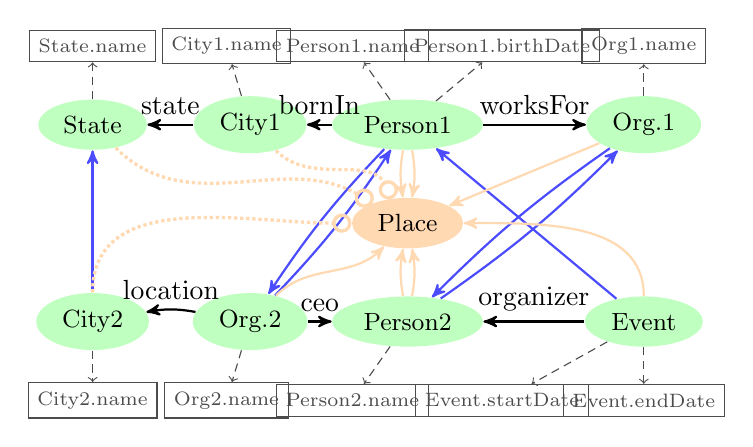
\begin{tikzpicture}

	\node[class] (pe1) at (3,0)  {\small Person1};
	\node[class] (co1) at (6,0) {\small Org.1};
	\node[class] (ci1) at (1,0) {\small City1};
	\node[class] (st1) at (-1,0) {\small State};
	
	\node[data] (pen) at (2.3,1) {\scriptsize Person1.name};
	\node[data] (peb) at (4.2,1) {\scriptsize Person1.birthDate};
	\node[data] (cin) at (0.7,1) {\scriptsize City1.name};
	\node[data] (stn) at (-1,1) {\scriptsize State.name};
	\node[data] (con) at (6,1) {\scriptsize Org1.name};
	
		
	\path[hasaC,->] (pe1) edge [bend left= 0] 
	node [midway, above, sloped] {worksFor} (co1) ;
	
	
	\path[hasaC,->] (pe1) edge [bend left = 0] 
	node [midway, above, sloped] {bornIn} (ci1) ;
	
	
	\path[hasaC,->] (ci1) edge  []
	node [midway, above, sloped] {state} (st1) ;

	

	\path[draw,hasaA,->] (pe1) -- (pen);
	\path[draw,hasaA,->] (pe1) -- (peb);	
	
	\path[draw,hasaA,->] (co1) -- (con);
	
	\path[draw,hasaA,->] (ci1) -- (cin);
	
	\path[draw,hasaA,->] (st1) -- (stn);


% % % CC2
\def\ysh{-2.5};

	\node[class] (pl2) at (-1,0+\ysh)  {\small City2};
	\node[class] (pe2) at (3,0+\ysh)  {\small Person2};
	\node[class] (co2) at (1,0+\ysh) {\small Org.2};
	\node[class] (ev2) at (6,0+\ysh) {\small Event};
	
	\node[data] (pen) at (2.3,-1+\ysh) {\scriptsize Person2.name};
	\node[data] (evs) at (4.2,-1+\ysh) {\scriptsize Event.startDate};
	\node[data] (eve) at (6,-1+\ysh) {\scriptsize Event.endDate};
	\node[data] (con) at (0.7,-1+\ysh) {\scriptsize Org2.name};
	\node[data] (pln) at (-1,-1+\ysh) {\scriptsize City2.name};
	
		
	\path[hasaC,->] (co2) edge [bend left= 0] 
	node [midway, above, sloped] {ceo} (pe2) ;
	
	
	\path[hasaC,->] (ev2) edge [bend left = 0] 
	node [midway, above, sloped] {organizer} (pe2) ;
	
	\path[hasaC,->] (co2) edge [bend left = -10] 
	node [midway, above, sloped] {location} (pl2) ;



	\path[draw,hasaA,->] (pl2) -- (pln);	

	\path[draw,hasaA,->] (pe2) -- (pen);
	
	\path[draw,hasaA,->] (co2) -- (con);
	
	\path[draw,hasaA,->] (ev2) -- (evs);
	\path[draw,hasaA,->] (ev2) -- (eve);
	

% % % Ontology

	\path[draw,hasaC,->,blue!70] (co2)  edge [bend left = -5] (pe1);
	\path[draw,hasaC,->,blue!70] (pe1)  edge [bend left = -5] (co2);
	
	\path[draw,hasaC,->,blue!70] (co1)  edge [bend left = -5] (pe2);
	\path[draw,hasaC,->,blue!70] (pe2)  edge [bend left = -5] (co1);

	\path[draw,hasaC,->,blue!70] (pl2) -- (st1);
	
	\path[draw,hasaC,->,blue!70] (ev2) -- (pe1);
	
	
	\node[class,fill=orange!30!white] (PL) at (3,\ysh/2)  {\small Place};
	
	\path[draw,hasaC,->,orange!30!white] (pe1) edge[bend left=10] (PL);
	\path[draw,hasaC,->,orange!30!white] (pe1) edge[bend left=-10] (PL);
	
	\path[draw,hasaC,->,orange!30!white] (pe2) edge[bend left=10] (PL);
	\path[draw,hasaC,->,orange!30!white] (pe2) edge[bend left=-10] (PL);
	
	\path[draw,hasaC,->,orange!30!white] (co1) edge[bend left=0] (PL);
	\path[draw,hasaC,->,orange!30!white] (co2) edge[out=45,in=225] (PL);

	\path[draw,hasaC,->,orange!30!white] (ev2) edge[out=90,in=0] (PL);
	
	\path[draw,isa,->,orange!30!white] (ci1) edge[out=-45,in=120] (PL);
	\path[draw,isa,->,orange!30!white] (pl2) edge[out=90,in=180] (PL);
	\path[draw,isa,->,orange!30!white] (st1) edge[out=-45,in=150] (PL);

\end{tikzpicture}
\caption{Example of alignment graph (`\tikz{ \node[class] () at (0,0)  
{};}' and `\tikz{ \node[class,fill=orange!30!white] () at (0,0)  
{};}' are class nodes, and `\tikz{ \node[data] () at (0,0)  {};}' are data 
nodes). We omit weights for clarity.}
\label{FIG:ali}
\end{figure}


\subsection{Frequent Subgraph Pattern Mining \label{SSEC:pattern-mining}}

As an extension to the problem, we consider using pattern mining techniques in 
order to identify patterns in the training set of semantic model that repeat 
themselves often. The hope is that with such information we can encourage the 
semantic model $m^\star$ for the new source to use groups of edges that 
appeared often together in training semantic models.

In our context, we define a \emph{pattern} is a graph $P$ that is undirected 
and simple (no multiple edges between two nodes, nor self-loops).

Let $G = (V_G,E_G,\lambda_G)$ and $P = (V_P,E_P, \lambda_P)$ be two graphs 
where $\lambda_G$ (resp. $\lambda_P$) is a \emph{labeling function} that maps 
nodes/edges of $G$ (resp. $P$) into a set of labels (e.g. natural numbers).
An \emph{embedding} of $P$ into $G$ is an injective function $f : V_G \mapsto 
V_P$ such that for all $x,y \in V_P$:
\begin{enumerate}
	\item $\{x,y\} \in E_P \implies \{f(x),f{y}\} \in E_G$.
	\item $\lambda_P(x) = \lambda_G(f(x))$
	\item $\lambda_P(\{x,y\}) = \lambda_G(\{f(x),f(y)\})$
\end{enumerate} 
That is, if an edge exists in $P$, it must also exist in $G$ (but not 
vice-versa); and the labelling functions of both graphs must match after 
applying the embedding function.

Our goal is to take a set of graphs (the semantic models from the training set 
$S_T$) and find patterns that appear often across that set of graphs. This is 
known as the Frequent Subgraph Mining (FSM), which contains the subgraph 
isomorphism, known to be NP-complete. 
There exists a range of tools that can achieve this task using Transactional 
Frequent Graph Pattern Mining
\cite{petermann2017dimspan,yan2002gspan}. We chose to use DIMSpan 
\cite{petermann2017dimspan}. \ddg{CHECK! How do they solve an NP-complete 
problem??}

This tool provides us with a list of patterns that are frequent, as well as 
their support. The \emph{support} of a pattern is a measure of frequency. Thus 
the higher the support, the more often the pattern appears. This typically 
means that big patterns have low support.

 

\section{Steiner Tree Formulation \label{SEC:STP}}

Given a graph $G =
(V, E)$ and a subset of its nodes $T \subseteq V$ , called \emph{terminals}, a 
Steiner Tree $G_s = (V_s, E_s )$ is a tree such that $T \subseteq V_s \subseteq 
V$ and $E_s \subseteq E$. In other words, $G_s$ spans all the nodes in $T$ and 
may include additional nodes from $V$, in particular to ensure the 
connectedness of the constructed tree. The Steiner Tree Problem 
(STP) is stated as follows: given $G$ and a weight function $w_f : E 
\mapsto \mathbb{R}$, find the Steiner Tree that minimizes the sum of the 
weights of the edges in $E_s$ given by $w_f$. This was proven to be NP-hard 
by Karp \cite{Karp1972}.

To formulate the \relonto{} schema mapping problem as a STP for a new source 
$s^\star$, we construct the 
\emph{integration graph} $~\mathcal{I}_\mathcal{O}^{s^\star} = 
(\mathcal{V}_\mathcal{O}^{s^\star},\mathcal{E}_\mathcal{O}^{s^\star})$, with 
nodes $\mathcal{V}_\mathcal{O}^{s^\star} = \mathcal{V_O} \cup 
\mathcal{A}_{s^\star}$, 
edges $\mathcal{E}_\mathcal{O}^{s^\star}$.

The set of edges $\mathcal{E}_\mathcal{O}^{s^\star}$ is constructed by using 
all the edges in the alignment 
graph, and edges connecting each attributes of $s^\star$ to the nodes in the 
alignment graph \emph{induced} by the semantic types (i.e. the set of nodes in 
$\mathcal{D_{G_O}}$). We call this last set 
of edges $\mathcal{M}_\mathcal{O}^{s^\star}$ (for ``matches''). Thus, 
$\mathcal{E}_\mathcal{O}^{s^\star} = 
\mathcal{E_O} \cup \mathcal{M}_\mathcal{O}^{s^\star}$.

We associate a weighting function  $w_\mathcal{I} : E \mapsto \mathbb{R}^+$ to 
the integration graph. For an edge $e \in \mathcal{E_O}$, $w_\mathcal{I}(e) = 
w_\mathcal{O}(e)$. For an edge $e 
\in \mathcal{M}_\mathcal{O}^{s^\star}$ connecting attribute $a_i$ to the node 
$l_j$ induced by the semantic model, $w_\mathcal{I}(e) = - 
ln(\psi(a_i,l_i))$. \ddg{CHECK!}

An example of integration graph can be found in Fig. \ref{FIG:inte}.




\begin{figure}[ht]
\centering
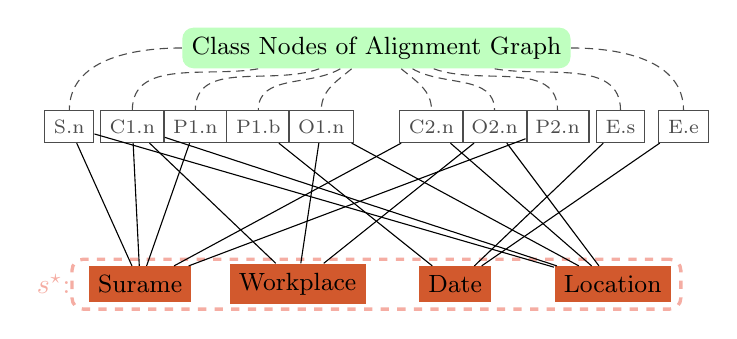
\begin{tikzpicture}
	\node[class, rectangle, rounded corners] (CLASS) at (0,0) { \small{Class 
	Nodes of Alignment Graph}};
	
	\node[data] (stn1) at (-3.9,-1) {\scriptsize S.n};
	\node[data] (cin1) at (-3.1,-1) {\scriptsize C1.n};
	\node[data] (pen1) at (-2.3,-1) {\scriptsize P1.n};
	\node[data] (peb1) at (-1.5,-1) {\scriptsize P1.b};
	\node[data] (con1) at (-0.7,-1) {\scriptsize O1.n};
	
	\path[draw,hasaA] (CLASS) edge[out=180,in=90] (stn1);
	\path[draw,hasaA] (CLASS) edge[out=190,in=90] (cin1);	
	\path[draw,hasaA] (CLASS) edge[out=200,in=90] (pen1);
	\path[draw,hasaA] (CLASS) edge[out=210,in=90] (peb1);	
	\path[draw,hasaA] (CLASS) edge[out=220,in=90] (con1);


% % % CC2
\def\ysh{0};
	
	\node[data] (cin2) at (0.7,-1+\ysh) {\scriptsize C2.n};
	\node[data] (con2) at (1.5,-1+\ysh) {\scriptsize O2.n};
	\node[data] (pen2) at (2.3,-1+\ysh) {\scriptsize P2.n};
	\node[data] (evs2) at (3.1,-1+\ysh) {\scriptsize E.s};
	\node[data] (eve2) at (3.9,-1+\ysh) {\scriptsize E.e};
	
	\path[draw,hasaA] (CLASS) edge[out=320,in=90] (cin2);	
	\path[draw,hasaA] (CLASS) edge[out=330,in=90] (con2);
	\path[draw,hasaA] (CLASS) edge[out=340,in=90] (pen2);
	\path[draw,hasaA] (CLASS) edge[out=350,in=90] (evs2);
	\path[draw,hasaA] (CLASS) edge[out=360,in=90] (eve2);
	
\node[rectangle, rounded corners,very thick,draw, dashed, 
brown!40!red!40!white,minimum 
height=18, minimum 
width=220] 
(source) at 
(0,-3) 
{};
\node[brown!40!red!40!white] 
(source) at 
(-4.1,-3) 
{$s^\star$:};
	\node[att] (a1) at (-3,-3) {\small Surame};
	\node[att] (a2) at (-1,-3) {\small Workplace};
	\node[att] (a3) at (1,-3) {\small Date};
	\node[att] (a4) at (3,-3) {\small Location};

	\path[draw] (a1) -- (stn1);
	\path[draw] (a1) -- (cin1);
	\path[draw] (a1) -- (pen1);
	\path[draw] (a1) -- (cin2);
	\path[draw] (a1) -- (pen2);
	
	\path[draw] (a2) -- (cin1);
	\path[draw] (a2) -- (con1);
	\path[draw] (a2) -- (con2);

	\path[draw] (a3) -- (peb1);
	\path[draw] (a3) -- (evs2);
	\path[draw] (a3) -- (eve2);

	\path[draw] (a4) -- (stn1);
	\path[draw] (a4) -- (cin1);
	\path[draw] (a4) -- (con1);
	\path[draw] (a4) -- (cin2);
	\path[draw] (a4) -- (con2);
\end{tikzpicture}
\caption{Example of integration graph. (`\tikz{ \node[att] () at (0,0)  
{};}' are attribute nodes). We omit weights for clarity. Data node labels are 
abbreviated but 
correspond to the ones shown in Fig \ref{FIG:ali}.}
\label{FIG:inte}
\end{figure}

Note that, although the alignment graph is directed, the semantic models are 
not necessarily rooted directed trees (e.g. Fig. \ref{FIG:sem}), therefore the 
direction of the edges is ignored for the STP model (and are all treated as 
undirected edges). 

The goal is to build a subgraph $T^\star= (V^\star, E^\star)$ 
of the integration graph 
$\mathcal{I}_\mathcal{O}^{s^\star}$ for the new source $s^\star$. The solution 
$T^\star$ will 
be used to build the source description $\delta^\star = (s^\star, m^\star, 
\phi^\star)$. 
In particular, $(\mathcal{V_O} \cap V^\star,\mathcal{E_O} \cap E^\star)$ 
corresponds to the semantic model, and 
$(\mathcal{A}_{s^\star},\mathcal{M}_\mathcal{O}^{s^\star} \cap E^\star)$ 
corresponds to 
the attribute mapping function.

The solution $T^\star$ must satisfy the following constraints:
\begin{enumerate}
	\item $T^\star$ must be a subgraph of $\mathcal{I}_\mathcal{O}^{s^\star}$
	\item $T^\star$ must be a tree (connected acyclic graph)
	\item $\forall a \in \mathcal{A}_{s^\star}, a\in V^\star$
	\item $\forall a \in \mathcal{A}_{s^\star}, degree(a) = 1$
	%\item $\forall n \in \mathcal{D_{G_O}}, degree(a) \in 
	%\{0,2\}$
	\item $\forall n \in \mathcal{D_{G_O}} \cap V^\star, 
	degree(a) = 2$
\end{enumerate}

It is therefore natural to model this a STP with side constraints, since the 2 
first requirements imply that $T^\star$ is a Steiner Tree of the integration 
graph. By designing the weighting function $w_\mathcal{I}$ through ML 
techniques, as shown in Section \ref{SEC:ML}, 
our hope is that the minimum weight Steiner Tree is a valid semantic model for 
the new source.


\subsection{Using Patterns}

As explained in Subsection \ref{SSEC:pattern-mining}, we also tried to use 
frequently appearing patterns in order to incentivise the solution tree 
$T^\star$ to contain subgraphs of the alignment graph that have been frequently 
seen in the training set.

To do this, we use the support of each of the obtained patterns as a prize. If 
the tree contains a pattern, then its weight is automatically reduced by a the 
value of the support of that pattern. We will see in the next section how this 
information is integrated in the model.

\subsection{Unmatched Attributes}
It is common that the data sources to be integrated will have columns that 
simply can't be matched to the ontology.
This can happen when a column of a source table contains some information that 
is uninteresting to the user, or because the ontology has not been properly 
designed. 
Examples of these situations can be found in domain specific data 
\cite{Pham2016} or HTML 
tables \cite{ritze2017matching}. In current systems, these columns are removed 
in a reprocess that requires extra time and effort as this is typically done 
manually in the real world.

For this reason, we add two artificial Class nodes to the integration graph:  
\emph{unknown} and \emph{root}. 
The latter will be connected to every other Class node in 
$\mathcal{V}_\mathcal{O}^{s^\star}$, including \emph{unknown}.
We also add a set $U = \{unk_1,...,unk_{|\mathcal{A}_{s^\star}|}\}$ of 
$|\mathcal{A}_{s^\star}|$ data 
nodes to the integration graph each connected to exactly one node in 
$\mathcal{A}_{s^\star}$ and to the \emph{unknown} Class node.  

If an attribute $a$ is matched to $unk_a$, then $unk_a$ will be linked to Class 
node \emph{unknown}. The rest of the attributes can then be matched normally 
and build  a semantic model as usual. Then, to maintain connectedness of the 
Steiner tree, the \emph{unknown} node and one of the selected Class nodes will 
both be connected to the \emph{root} node. Note that if all attributes find a 
match, then both the \emph{unknown} and \emph{root} won't be selected in the 
Steiner tree and the normal behavior will take place.
\ddg{Explain the weights of the edges introduced by the unknown nodes}




\section{Modeling as a Constraint Optimization Problem \label{SEC:CP}}

\subsection{Definitions}
A Constraint Satisfaction Problem (CSP) is a tuple $P = (\boldsymbol{v},D,C)$ 
where $\boldsymbol{v}$ is a 
set of \emph{variables}, $D$ is a set of unary constraints over 
$\boldsymbol{v}$ specifying 
the \emph{domain} of these variables, $C$ is a set of $n$-ary 
\emph{constraints} over variables $\boldsymbol{v}$.
A valuation $\theta(\boldsymbol{v})$ is a mapping from the set of variables to 
values in $D$. If there exist a valuation $\theta^\star$ such that all 
variables map 
to exactly one value, and all the constraints in $D\cup C$ are satisfied by the 
valuation, then $\theta^\star$ is a \emph{solution} to $P$.

A Constraint Optimization Problem (COP) is a CSP with an additional 
\emph{objective function} $o : \boldsymbol{v} \mapsto \mathbb{R}$ and a 
\emph{sign} which is either \verb|minimize| or \verb|maximize|. 

A typical example of COP is the Traveling Salesman Problem, where we need to 
find a route that visits all cities in a region exactly one and is of minimal 
length.

\subsection{Constraint Programming}
Constraint Programming (CP) allows the user to model a CSP or COP and give it 
to a 
solver that will find a solution to the CSP, or will report unsatisfiability if 
no solution exists. In the case of COPs, the solver will try to optimize 
the objective function and prove optimality as well.

Briefly, the way a CP solver works is by assigning a value to each variable of 
$\boldsymbol{v}$ from $D$ in turn. At each iteration it will check whether any 
constraint in $C$ is violated, in which case it will backtrack to change it's 
last decision. The choice of the order of the variables to be assigned, and the 
choice of the value to be assigned to each variable is called the \emph{search 
strategy}.

Since only using a backtracking algorithm would have a prohibitive cost, CP 
uses a combination of search and \emph{propagation}. The latter is achieved by 
\emph{propagating} the last decision made via specialized algorithms called 
\emph{propagators}. A propagator is a function $p : (v, D_v) \mapsto D_v'$ that 
takes a subset of the variables of the problem $v \subseteq \boldsymbol{v}$ and 
the domain of those variables $D_v$ and returns a new domain for these 
variables 
such that $D_v' \sqsubseteq D$. That is, a propagator removes values form the 
domains of variables (when possible). For a propagator to be correct, it must 
not remove a value of the domain of a variable if such value could participate 
in a solution given the decisions already made.

\emph{Global constraints} are higher order constraints that enforce a 
complicated 
constraint over a set of variables. Typical examples of this is enforcing that 
a set of variables take different values, or that they describe a path a in a 
graph. Although it is possible to express these constraints with a conjunction 
of simple constraints, it is often the case that specific algorithms for these 
constraints perform substantially better than a decomposition approach (e.g. 
\cite{regin1994filtering}). A wide 
list of these global constraints can be found in \cite{beldiceanu2012global}.

\subsubsection{Example} Consider the toy problem $P$ over variables $a$ and $b$ 
such that $a \in \{2,3,4\}$, $b \in \{1,2,3\}$. Let $C = \{a + 2b \leq 4, a 
\neq b\}$ be the constraints. If the search step decides that $a = 
2$, then $(i)$ $a \neq b \Rightarrow b \in \{1,3\}$ and $(ii)$ $a + 2b \leq 4  
\Rightarrow b \in \{1\}$. Thus we automatically know that $b = 1$ without never 
trying any other of its original possible values. $\square$


\subsection{Modeling \relonto{} in CP}
In order to model this problem we used the \minizinc{} language 
\cite{minizinc}, and the 
\chuffed{} solver \cite{chu2011improving} because it has a global constraint 
implemented for Steiner 
Tree Problems \cite{deuna2016steiner}. 

Because attributes must be connected to exactly one node of the alignment 
graph, and that node will be in $\mathcal{D_{G_O}} \cap V^\star$ 
then the part of the problem between attribute nodes and the alignment graph is 
actually a matching problem. Each attribute must match exactly to one node of 
$\mathcal{D_{G_O}}$. Note that not all nodes in $\mathcal{D_{G_O}}$ must match 
to an attribute, as not all of them are part of $T^\star$.

Because there are global constraints in CP specialized in matching 
\cite{regin1994filtering}, we split the problem into two parts: the 
\verb|steiner_tree| global constraint will only deal with the part of the 
integration graph that corresponds to the alignment graph, and the 
\verb|alldifferent| global constraint will deal with he matching part of the 
problem.

We use the following variables to represent the tree $T^\star$: Boolean 
variables $c_n,\forall n \in 
\mathcal{V_O}$, $c_e, \forall e \in	\mathcal{E_O}$ and an array of variables 
$match$ indexed by the set of attributes of $s^\star$. The combination of these 
sets fo variables define the value of $T^\star$: $c_n = \mathit{true}$ means 
that $n \in V^\star$, $c_e = \mathit{true}$ means that $e \in E^\star$ and 
$match[a] = d$ (for $a \in \mathcal{A}_{s^\star}$ and $d \in 
\mathcal{D_{G_O}}$) means that the edge $(a,d) \in 
\mathcal{M}_\mathcal{O}^{s^\star}$ is part of $T^\star$.

Additionally, for a given set of patterns $\mathcal{P}$ with a support function 
$w_\mathcal{P} : \mathcal{P} \mapsto \mathbb{R}$, we have a set of Boolean 
variables 
$c_p, \forall p \in \mathcal{P}$ that tells us whether a pattern $p$ appears in 
$T^\star$ or not.
The model is presented below.

\begin{flalign}
	& \text{Minimize~~} w_{STP} + w_{ADIFF} - w_{PAT}
	%\sum_{e \in \mathcal{E}_\mathcal{O}}c_e * 
	%w_\mathcal{I}(e) + \sum_{e \in \mathcal{M}_\mathcal{O}^{s^\star}} c_e * 
    %		w_\mathcal{I}(e)
	\label{EQ:obj}&&\\
	&\text{such that~~}  \nonumber&& \\
	& \textit{steiner}(\{c_n| n \in \mathcal{V_O}\},\{c_e| e \in 
	\mathcal{E_O}\},\mathcal{G_O},w_\mathcal{O},w_\mathit{STP})  \label{EQ:stp} 
	&&\\
	&\forall d \in \mathcal{D_{G_O}}, degree(d) \leq 1 \label{EQ:deg1}&&\\
	&\forall d \in \mathcal{D_{G_O}}, c_d \Leftrightarrow degree(d) = 1 
	\label{EQ:deg2}&&\\
	&\forall a \in \mathcal{A}_{s^\star}, match[a] \in \{ d | (a,d)\in 
	\mathcal{M}_\mathcal{O}^{s^\star} \} \label{EQ:matchdom}&&\\
	& \textit{alldifferent}(match) \label{EQ:alld}&& \\
	& \forall a \in \mathcal{A}_{s^\star}, c_{match[a]} = \mathit{true} 
	\label{EQ:map}&&\\
	& w_{\mathit{ADIFF}} = \sum_{(a,d) \in \mathcal{M}_\mathcal{O}^{s^\star}} 
	w_\mathcal{I}(~(a,d)~) * \llbracket match[a] = d\rrbracket 
	\label{EQ:matchcost}  &&\\
	& \forall p \in \mathcal{P}, \big(\forall e\in edges(p), c_e = 
	\mathit{true} \big) \Leftrightarrow c_p \label{EQ:patt}&&\\
	& w_{PAT} = \sum_{p\in\mathcal{P}} w_\mathcal{P}(p)* c_p 
	\label{EQ:pcost} &&\\
	& c_{unknown} \Rightarrow \big( c_{root}  \land 
	c_{(unknown,root)} \big) \label{EQ:unk}
\end{flalign}

Eq. \ref{EQ:obj} is the objective function: we are minimizing the cost 
of $T^\star$ while collecting prizes for each pattern we use. Eq. \ref{EQ:stp} 
enforces that the solution 
$T^\star$ is indeed a tree defined by the $c_n$ and $c_e$ variables, subgraph 
of the alignment graph 
and of total weight $w_{STP}$. Equations \ref{EQ:deg1} and \ref{EQ:deg2} ensure 
that if a data node of the alignment graph is selected, then at most one edge 
reaches it (from the side of the alignment graph) and otherwise it is 
disconnected. Eq. \ref{EQ:matchdom} ensures that the domain of each variable in 
the array $match$ corresponds to a subset of data nodes of the alignment graph 
for which there is an edge connecting to the attribute at hand. Eq. 
\ref{EQ:alld} ensure that each attribute is mapped to exactly one data node of 
the alignment graph. Equations \ref{EQ:matchdom} and \ref{EQ:alld} ensure that 
there is exactly one data node matched to an attribute, which has to be one of 
the ones for which an edge existed. Eq. \ref{EQ:map} ensures that 
if a data node of the alignment graph has been mapped to some attribute, then 
that data node must be in the solution tree, and vice-versa. Eq. 
\ref{EQ:matchcost} computes the cost $w_{ADIFF}$ of the matches.
Eq. \ref{EQ:patt} indicated that a pattern is used if and only if all its edges 
are selected in the tree. Eq. \ref{EQ:pcost} computes the prizes collected by 
using patterns.
Eq. \ref{EQ:unk} ensures that if the \emph{unknown} class node is used, then it 
is connected to \emph{root}.
Notice how there is no further requirement for unmatched attributes, as the 
$unk_i$ data nodes behave like normal data nodes, and the connectedness 
requirement will make sure that \emph{root} is connected to the rest of the 
tree (i.e. the semantic model).

Note how this CP model is easily adaptable to more classic settings where no 
patterns are used (by dropping Eqs. \ref{EQ:patt} and \ref{EQ:pcost}), or where 
the \emph{unknown} nodes are used (by dropping \ref{EQ:unk}).
\section{Results \label{SEC:Res}}

\subsection{Experimental Setup}
\ddg{TODO}

\subsection{Experimental Results}
\ddg{TODO}

\section{Conclusions}
\ddg{TODO} 


\bibliographystyle{aaai}
\bibliography{main}
\end{document}
